\section{Nurul Izza Hamka - 1174062}
\subsection{Teori}
\begin{enumerate}

\item Jelaskan kenapa file suara harus dilakukan MFCC, dilengkapi dengan ilustrasi atau gambar

Mel Frequency Cepstrum Coefficient (MFCC) adalah salah satu metode yang digunakan pada bidang speech recognition. Metode MFCC ini digunakan untuk melakukan feature extraction, yang mana sebuah proses yang mengkonversikan sinyal suara menjadi beberapa parameter. Metode MFCC memiliki keunggulan yaitu:\\
- Mempu menangkap karakteristik suara dan informasi-informasi yang sangat penting yang ada dalam sinyal suara.\\
- Mengurangi data seminimal mungkin, tapi tidak menghilangkan data dan informasi yang penting.\\
-Dapat mereplikasi organ pendengaran pada manusia dalam persepsi sinyal suara.

\begin{figure}
	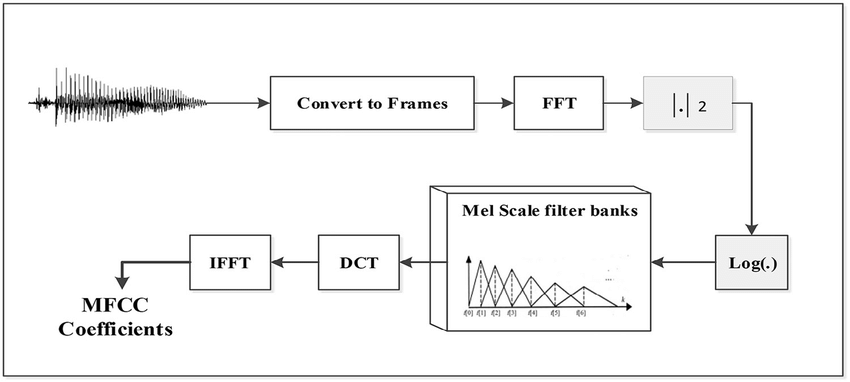
\includegraphics[width=4cm]{figures/1174062/6/no1.png}
	\centering
	\caption{Mel Frequency Cepstrum Coefficient}
\end{figure}

\item Jelaskan konsep Neural Network dilengkapi dengan ilustrasi atau gambar.

Ada beberapa konsep dari Neural Network yaitu:\\
- Proses kerja jaringan saraf pada otak manusia.\\
Ide dasar dari neural network ini dimulai dari otak manusia, yang mana otak memuat sekitar 1011  neuron. Satu neuron ini terdapat sat akson, dan min 1 dendrit.\\
- Struktur Neural network\\
Ide dasar dari Artifial Neural Network adalah mengadopsi mekanisme berpikir sebuah sistem atau aplikasi yang menyerupai otak manusia, baik untuk pemrosesan berbagai sinyal.\\

\begin{figure}
	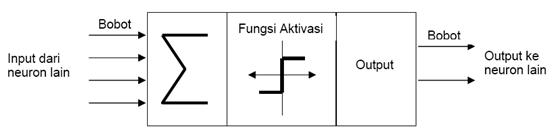
\includegraphics[width=4cm]{figures/1174062/6/2.png}
	\centering
	\caption{Konsep Dasar Neural Network}
\end{figure}

Dari gambar di atas berikut penjelasannya:\\
a.	Input, sebagai dendrite\\
b.	Output, sebagai akson\\
c.	Fungsi aktivasi, sebagai sinapsis\\

\item Jelaskan konsep pembobotan dalam neural network dilengkapi denan ilustrasi atau gambar.

Fleksibilitas yang dimiliki neural network adalah pemilihan input model, fungsi aktivasi yang digunakan dan juga pemilihan metode optimasi pada jaringan untuk mendapatkan bobot yang optimal. Bobot-bobot dalam Neural network biasanya diinisialisasi secara random dengan nilai random yang kecil. Jika dalam inisialisasi nilai bobot random yang diperoleh jauh dari solusi yang baik, atau dekat dengan nilai yang optimum local yang masih kurang baik, maka proses training akan cukup lama.

\begin{figure}
	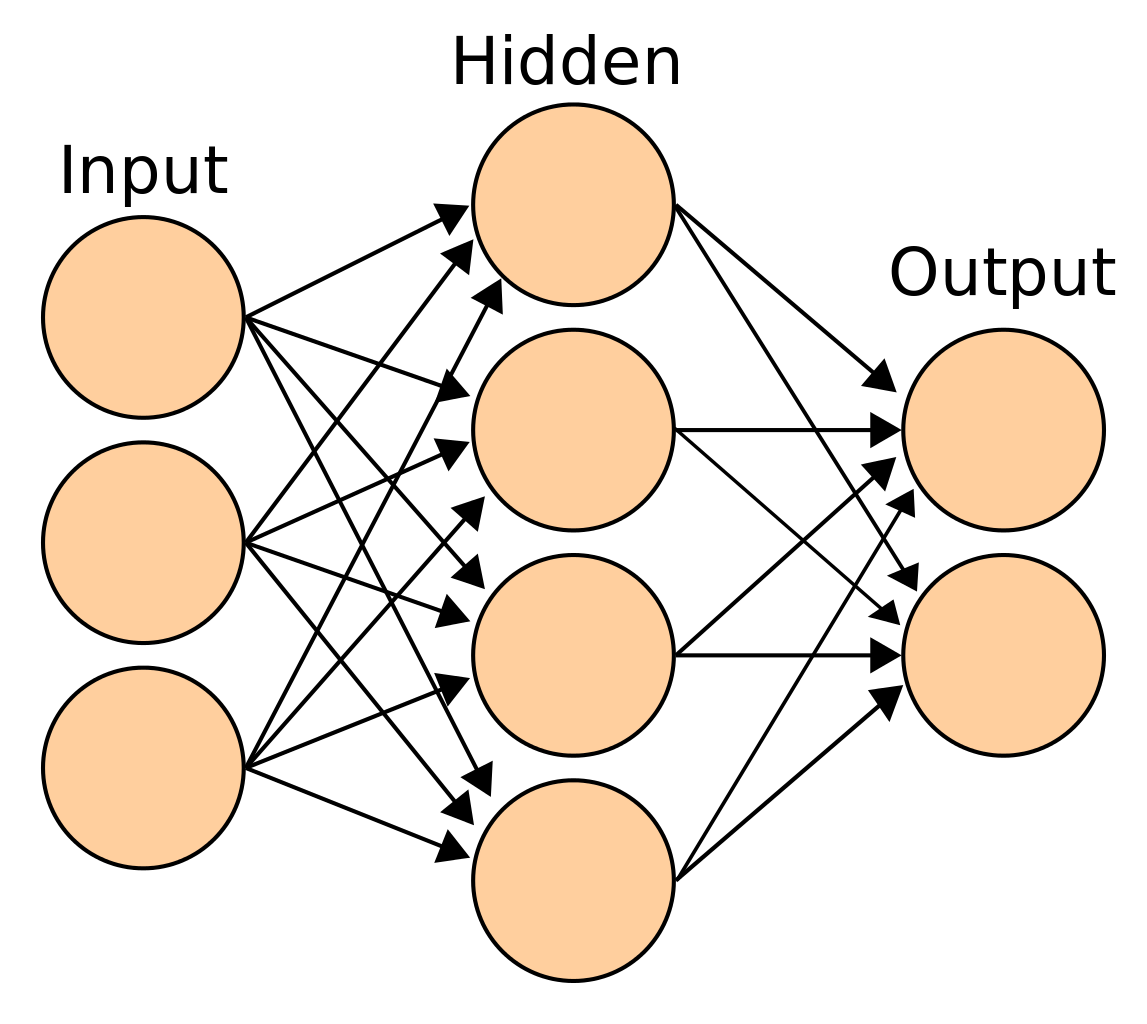
\includegraphics[width=4cm]{figures/1174062/6/no3.png}
	\centering
	\caption{Konsep Pembobotan Neural Network}
\end{figure}

\item Jelaskan konsep fungsi aktifasi dalam neural network, dilengkapi dengan ilustrasi atau gambar

Fungsi aktifasi dalam neural network adalah fungsi matematis yang digunakan untuk mendapatkan sebuah output neuron dari nilai yang diinputkan. Ada bebrapa fungsi aktifasi yang sering digunakan yaitu: hard limiter, signum activation dan sigmoid activation. Pada perceptron, fungsi aktifasi ini hanya terdapat pada neuron yang ada di output layer.

\begin{figure}
	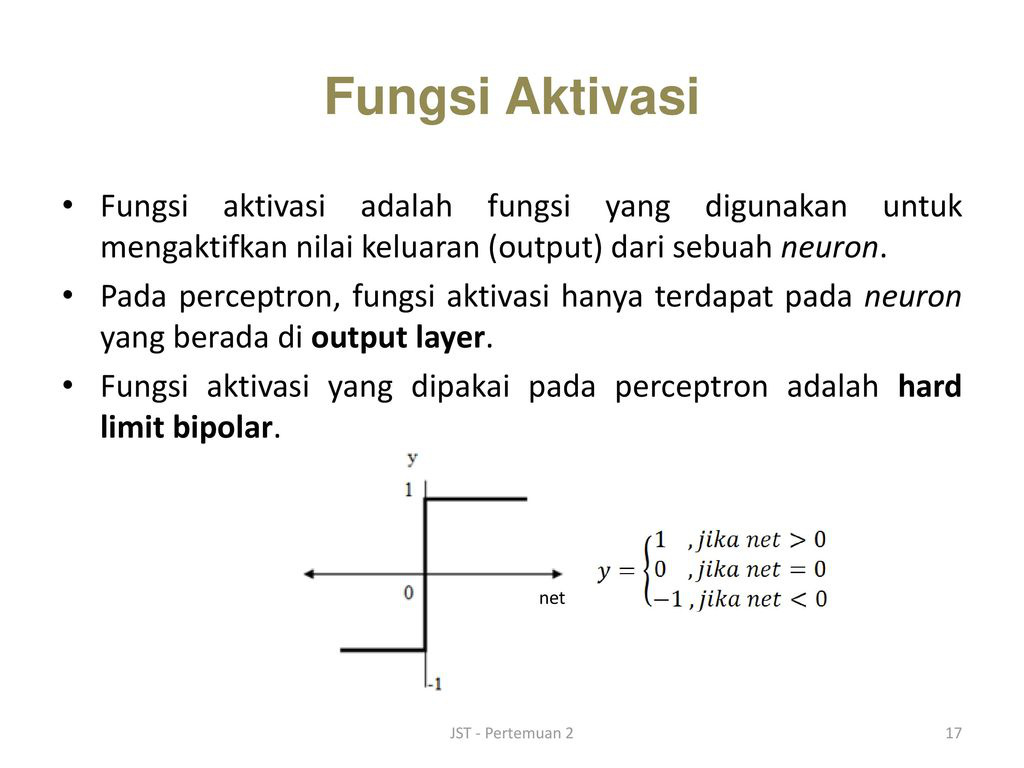
\includegraphics[width=4cm]{figures/1174062/6/no4.png}
	\centering
	\caption{Fungsi Aktifasi Neural Network}
\end{figure}

\item Jelaskan cara membaca asil plot dari MFCC dilengkapi dengan ilustrasi atau gambar sendiri.

\begin{figure}
	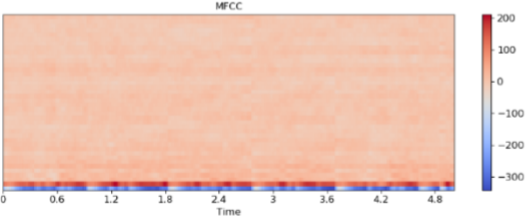
\includegraphics[width=4cm]{figures/1174062/6/no5.png}
	\centering
	\caption{Plot MFCC}
\end{figure}

Dari gambar diatas diketahui:\\
- Terdapat dua dimensi yaitu x (waktu) dan y (power dan disable),\\
- Jika berwarna artinya power dari suara tersebut berarti rendah, dan jika merah artinya suara tinggi,\\
- Sedangkan untuk warna merah yang agak pudar artinya tidak ada suara sama sekali.\\

\item Jelaskan apa itu one-hot encoding dilengkapi ilustrasi kode dan atau gambar

One-hot encoding adalah proses dimana variabel kategorikal dikonversi menjadi bentuk yang dapat disediakan untuk algoritma ML untuk melakukan pekerjaan yang lebih baik dalam prediksi.

\begin{figure}
	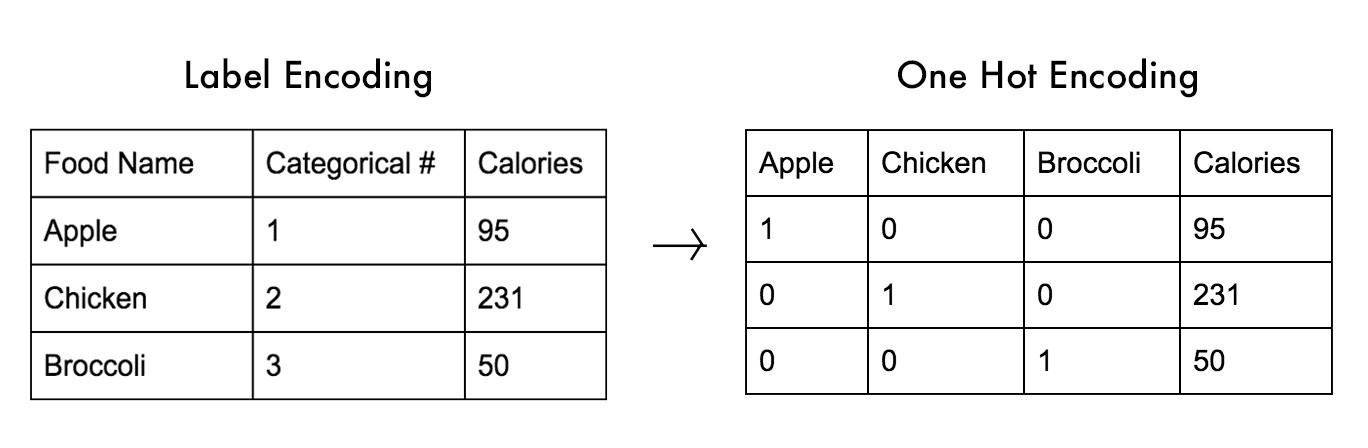
\includegraphics[width=4cm]{figures/1174062/6/no6.png}
	\centering
	\caption{One-Hot Encoding}
\end{figure}

\item Jelaskan apa fungsi dari np.unique dalam kode program dilengkapi dengan ilustrasi atau gambar.

Fungsi dari np unique sendiri adalah menemukan elemen unik dari array, dan juga mengembalikan sebuah elemen unik array yang telah diurutkan. Kemudian terdapat juga tiga output selain dari elemen unik yaitu:\\
- Indeks array input, yaitu untuk memberikan sebuah nilai yang unik,\\
- Indeks array unik, yaitu untuk melakukan rekontruksi array input tadi,\\
- Dan yang terakhir adalah beberapa kali setiap nilai unik muncul dalam array input tersebut.\\

\item Jelaskan apa fungsi dari sequential dalam kode program dilengkapi dengan ilustrasi atau gambar.
Sequential sendiri berfungsi sebagai tumpukan lincar lapisan.
\end{enumerate}

\subsection{Praktek Program}
\begin{enumerate}

\item Jelaskan isi dari data GTZAN Genre Collection dan data dari freesound. Buat kode program untuk meload data tersebur untuk digunakan pada MFCC.

	\hfill\break
	\lstinputlisting[firstline=8, lastline=30]{src/1174062/6/1174062.py}

\item Jelaskan perbaris kode program dengan kata-kata dan dilenkapi dengan ilustrasi gambar dari display mfcc.
	\hfill\break
	\lstinputlisting[firstline=32, lastline=54]{src/1174062/6/1174062.py}
	
\item Jelaskan perbaris kode program dengan kata-kata dan dilengkapi ilustrasi gambar fungsi dari extract feature song. Jelaskan mengapa yang diambil 25.000 baris pertama?

	\hfill\break
	\lstinputlisting[firstline=56, lastline=67]{src/1174062/6/1174062.py}

\item Jelaskna perbaris kode program dengan kata-kata dan dilengkapi ilustrasi gambar fungsi dari generate features and labels().

	\hfill\break
	\lstinputlisting[firstline=69, lastline=88]{src/1174062/6/1174062.py}

\item Jelaskan dengan kata dan praktek kanapa penggunaan fungsi generate feature and labels() sangat lama ketika meload dataset genre.

	\hfill\break
	\lstinputlisting[firstline=90, lastline=95]{src/1174062/6/1174062.py}

\item Jelaskan mengapa harus dilakukan pemisahan data training dan dataset sebesar 80 persen? Praktekkan dengan kode dan tunjukkan keluarannya.

	\hfill\break
	\lstinputlisting[firstline=97, lastline=116]{src/1174062/6/1174062.py}

\item Praktekkan dan jelaskan masing-masing parameter dari fungsi Sequential(). Tunjukkan keluarannya dari komputer sendiri.

	\hfill\break
	\lstinputlisting[firstline=119, lastline=126]{src/1174062/6/1174062.py}

\item Praktekkan dan jelaskan masing-masing parameter dari fungsi fit(). Tunjukkan keluarannya dengan fungsi summary dari komputer sendiri dan artikan maskud setiap luaran yang didapatkan.

	\hfill\break
	\lstinputlisting[firstline=128, lastline=133]{src/1174062/6/1174062.py}

\item Praktekkan dan jelaskan masing-masing parameter dari fungsi fit(). Tunjukkan keluarannya dari  komputer sendiri dan artikan maksud setiap luaran yang didapatkan.

	\hfill\break
	\lstinputlisting[firstline=135, lastline=138]{src/1174062/6/1174062.py}
	
\item Praktekkan dan jelaskan masing-masing parameter dari fungsi evaluate(). Tunjukkan keluarannya  dari komputer sendiri dan artikan maksud setiap luaran yang didapatkan.

	\hfill\break
	\lstinputlisting[firstline=140, lastline=145]{src/1174062/6/1174062.py}
	
\item Praktekkan dan jelaskan masing-masing parameter dari fungsi predict(). Tunjukkan keluarannya dari komputer sendiri dan artikan maksud setiap luaran yang didapatkan.

	\hfill\break
	\lstinputlisting[firstline=147, lastline=149]{src/1174062/6/1174062.py}

\end{enumerate}
\end{document}